\section{Dynamic Compensators and Stability Margins}

\subsection{Stability Margins}

Gain margin: factor by which the gain can be rained before a system becomes unstable.

Phase margin: The amount by which the phase can be increased before the system becomes unstable. (exceeds $-180 ^\circ$)


For a system to be robust the gain margin should be 3 to 6dB and the phase margin
should be $30^\circ$ to $45^\circ$.

The phase margin can be found on a bode plot by looking at the phase at the frequency
where the gain is 0dB. The phase margin is then $180^\circ$ minus the phase at that frequency.
The gain margin is the gain at the frequency where the phase is $-180^\circ$.


\begin{center}
	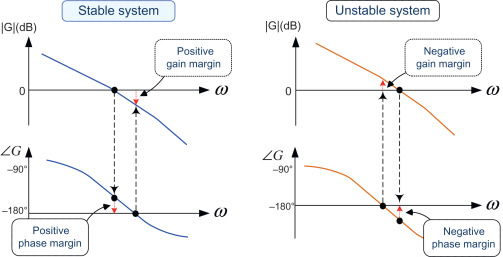
\includegraphics[width=0.7\textwidth]{Images/margin.jpg}
\end{center}

\subsection{Dynamic compensation}

Lead compensator is equivalent to a d-part for a PID controller.
A lead compensator has a positive phase. A lead compensater decreases
the rise time and overshoot.

Lag compensator is equivalent to an i-part for a PID controller.
The lag controller improves the steady state error.

Both compensators are given by the transfer function:

$$ D(s) = K \frac{s + z}{s + p} $$
Where $z$ and $p$ are the zero and pole of the transfer function respectively.

\begin{itemize}
	\item {If $z<p$, then $D(s)$ is called a lead compensation}
	      \item{If $z>p$, then $D(s)$ is called a lag compensation}
\end{itemize}

\subsubsection{Lead compensation}

Used for dynamic properties such as rise time, overshoot and settling time. It has relation
to the phase margin, where we can lift the phase margin by adding a lead compensator.

A lead compensation is given by:
$$D(s) = \frac{Ts+1}{\alpha Ts+1}$$
and $1/\alpha$ is called the lead ratio.

We have the following properties:
$$\omega_{max} = \frac{1}{T\sqrt{\alpha}} = \sqrt{|z||p|}$$,
$$T = \frac{1}{\omega_{max}\sqrt{\alpha}}$$
$$sin(\phi_{max}) = \frac{1-\alpha}{1+\alpha}$$

$\phi_{max}$ is the maximum phase lead. Which means that it is the
maximum phase that the lead compensator can provide.
And $\omega_{max}$ is the frequency at which the phase lead is maximum.


\begin{center}
	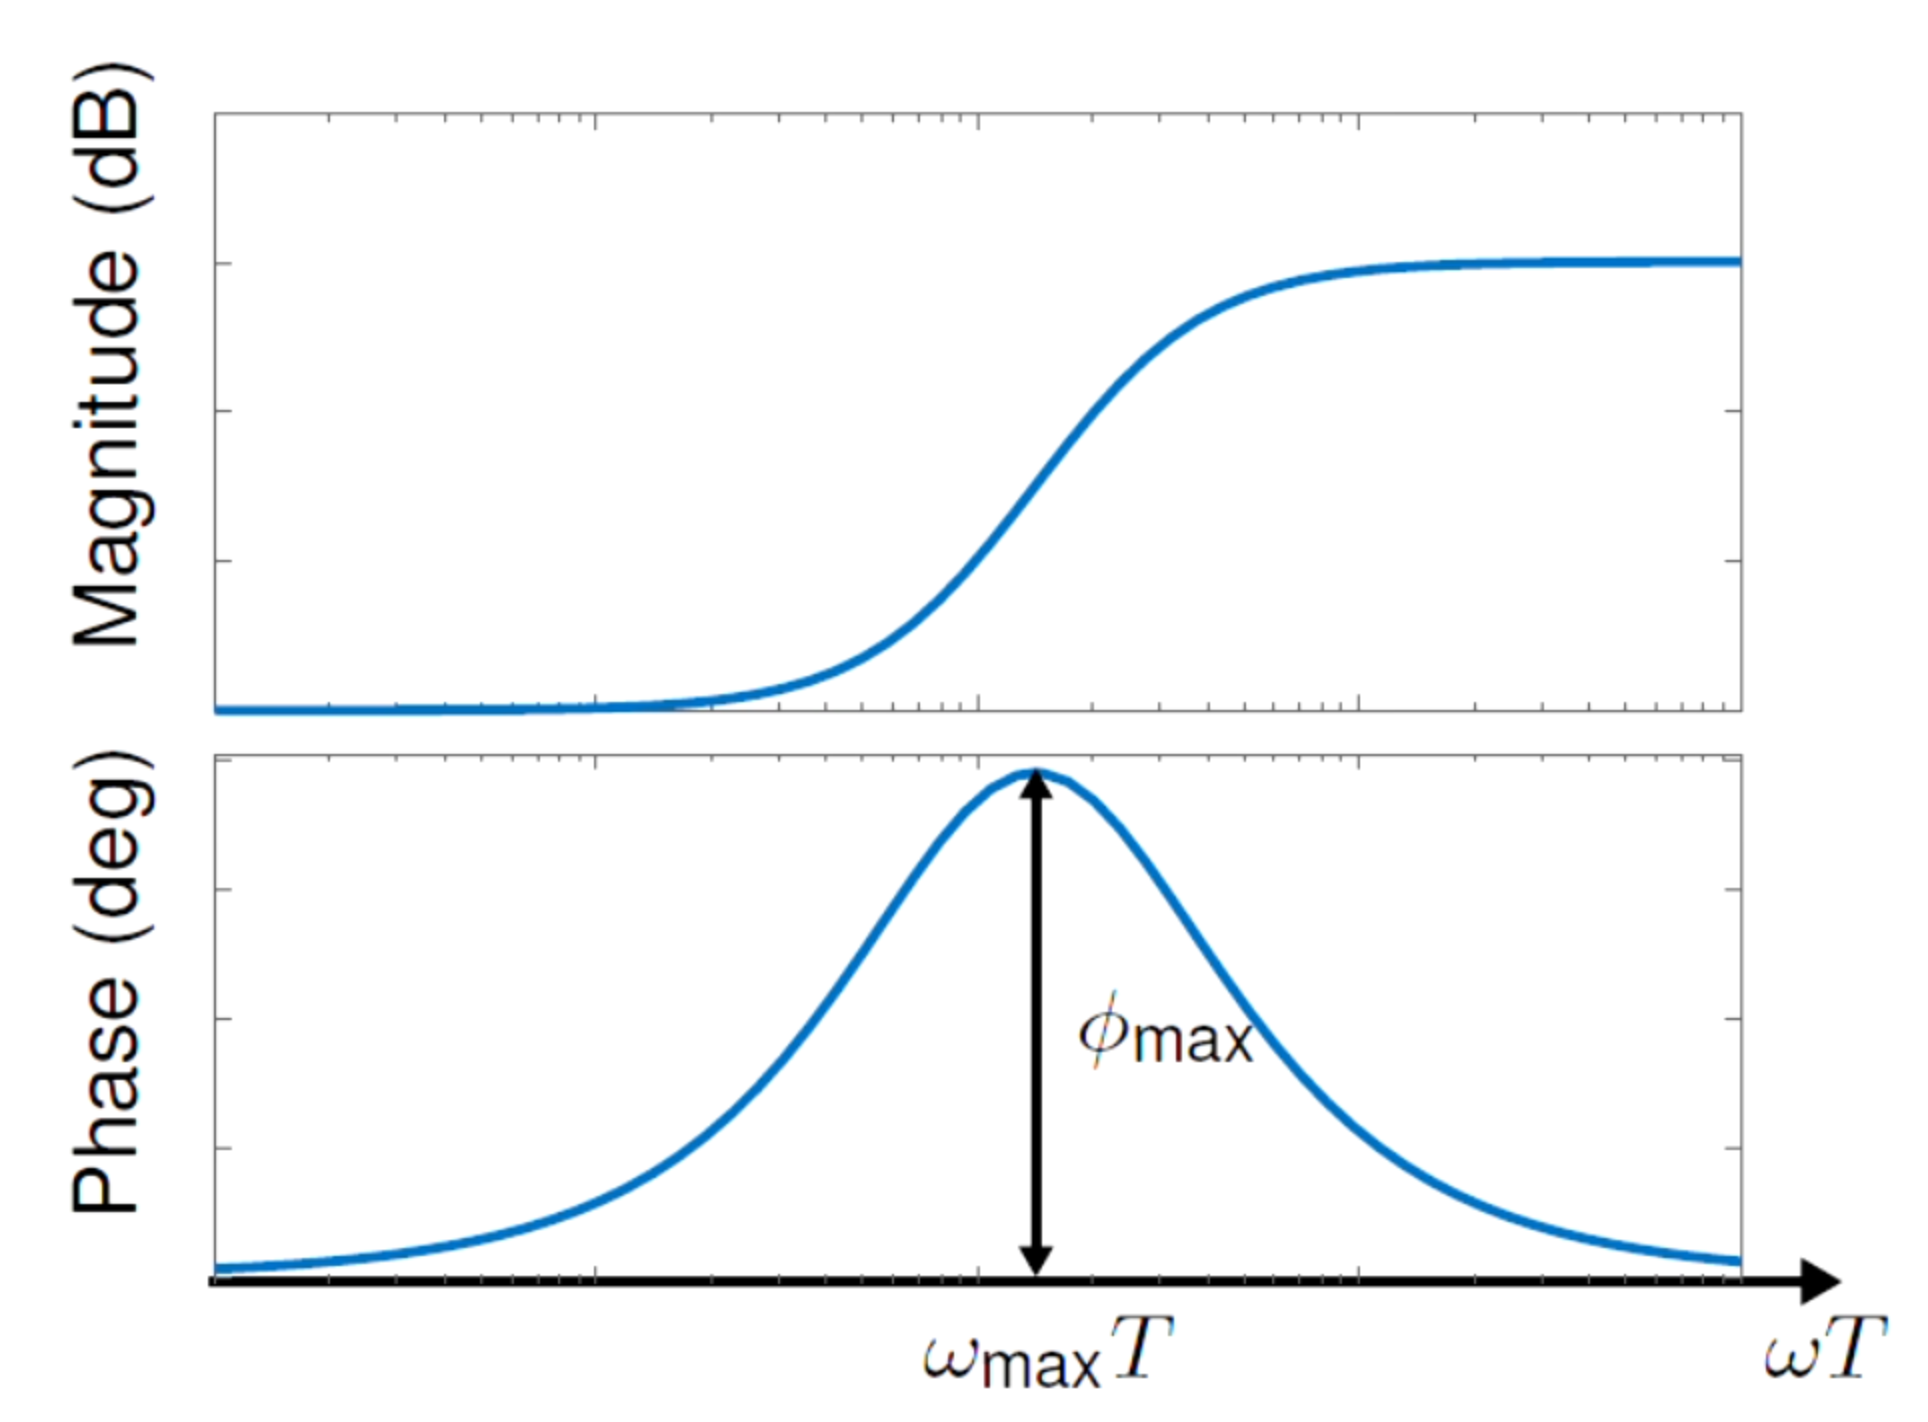
\includegraphics[width=0.5\textwidth]{Images/leadComp.png}
\end{center}

\subsubsection{Lag compensation}
A lag compensator can be used for minimizing the steady state error without affecting
the other dynamics. Only looking at stationary error. It doesn't eliminate the error
but reduces it.

A lag compensator can be written as:
$$D(s) = K_0 \frac{\alpha Ts+1}{\alpha Ts+1}$$
where $K_0$ is the gain of the compensator, $z>p \in \mathbb{R}$ and $\alpha > 1$.

The gain decreases and the phase gets negative.


\begin{center}
	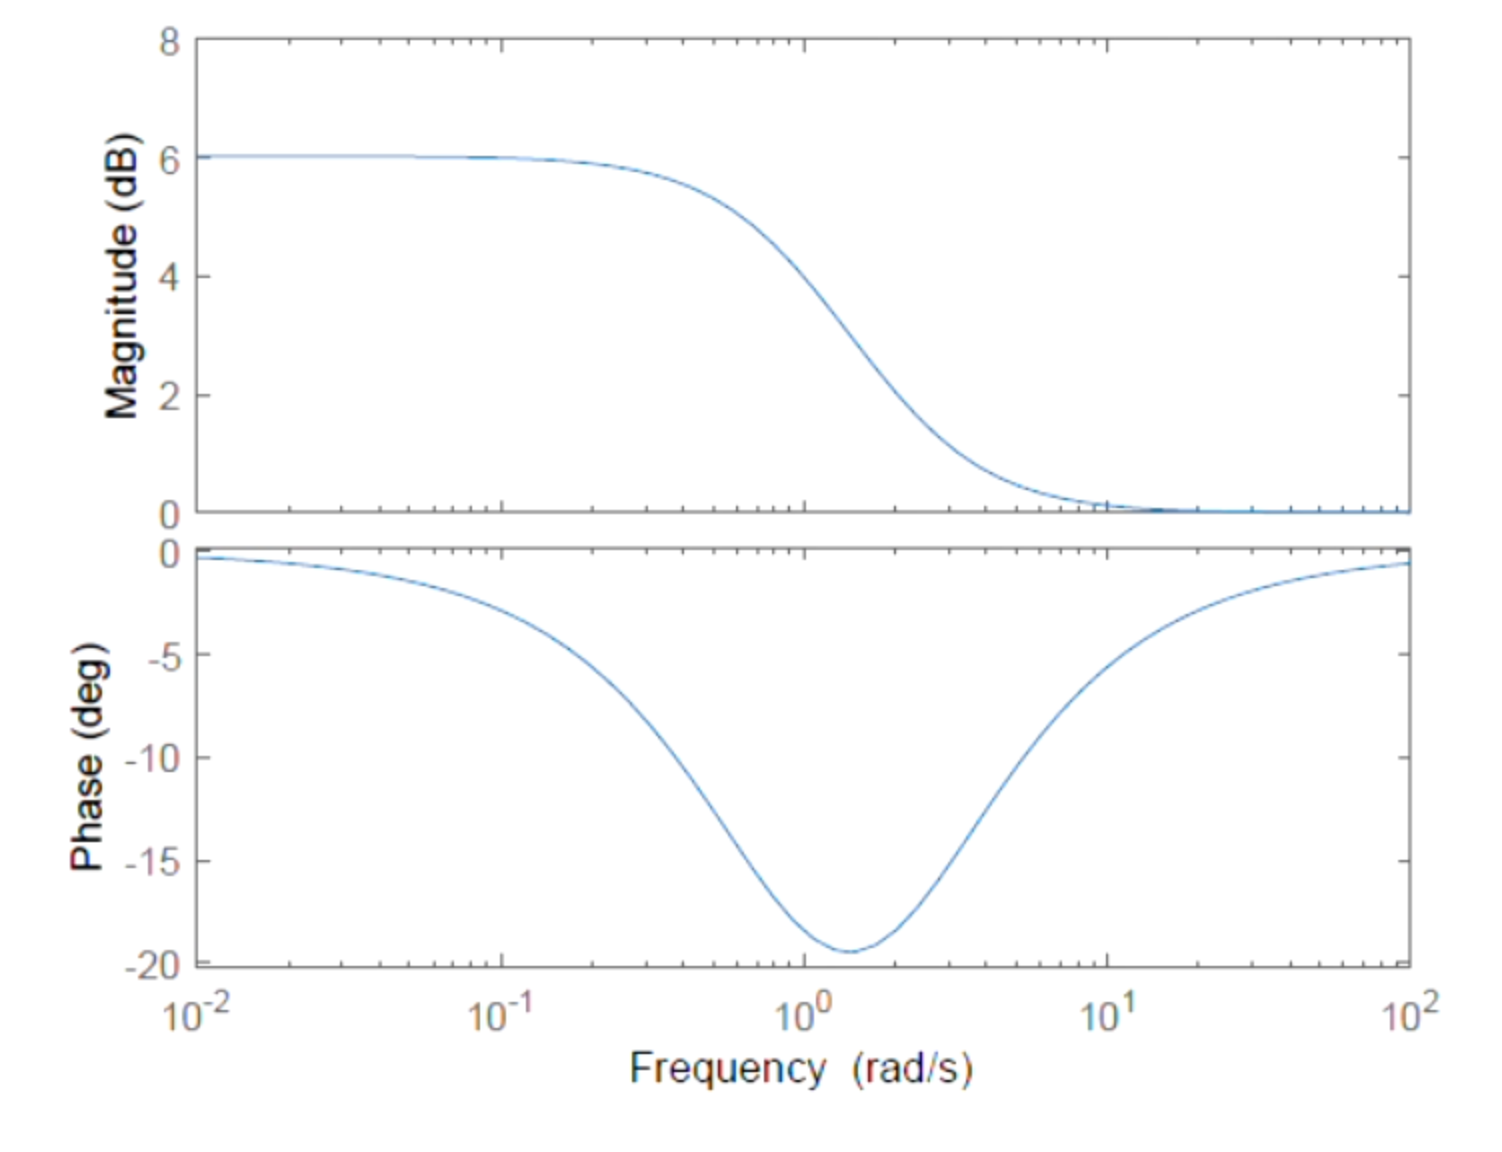
\includegraphics[width=0.5\textwidth]{Images/lagComp.png}
\end{center}

\subsection{Examples}
